\documentclass[11pt]{article}

\usepackage[a4paper,margin=2.45cm]{geometry}
\usepackage{amsmath,amssymb,amsthm,mathtools}
\usepackage{graphicx}
\usepackage{booktabs}
\usepackage{microtype}
\usepackage[hidelinks]{hyperref}
\usepackage{xcolor}
\usepackage{enumitem}

\newtheorem{proposition}{Proposition}[section]
\newtheorem{theorem}[proposition]{Theorem}
\newtheorem{remark}[proposition]{Remark}
\newtheorem{lemma}[proposition]{Lemma}
\newtheorem{definition}[proposition]{Definition}

\newcommand{\R}{\mathbb{R}}
\newcommand{\B}{\overline{B}_2(0,1)}
\newcommand{\dist}{\operatorname{dist}}
\newcommand{\conv}{\operatorname{conv}}
\newcommand{\sgn}{\operatorname{sgn}}

\title{A Nonconvex Planar Differential Inclusion with Two Rotating Disks\\
\large A relaxation-gap benchmark for hard selectors and distance residuals}
\author{}
\date{}

\begin{document}
\maketitle

\begin{abstract}
We describe a two-dimensional nonconvex differential inclusion obtained by replacing the rotating ellipse of a previous benchmark with the union of two disjoint rotating disks. The example is designed so that a prescribed terminal state is generated by the relaxed selector $\xi\equiv 0$, which belongs to the convex hull of the admissible set but not to the admissible set itself. Consequently, exact admissible trajectories can approach the target only through increasingly rapid switching between the two components. The example gives a transparent numerical realization of the Filippov--Wazewski relaxation mechanism and exposes the precise point at which a convex consistency argument for distance-residual methods fails. We compare a hybrid selector parametrization that is admissible by construction with a smooth, unconstrained distance-residual formulation. The former reaches the target through chattering while keeping the inclusion residual identically zero; the latter reaches essentially the same terminal state but exhibits either residual spikes at component crossings or a positive residual plateau inside the nonconvex gap.
\end{abstract}

\section{The nonconvex differential inclusion}

Let $T>0$, $J=[0,T]$, and consider trajectories $x:J\to\R^2$ governed by
\begin{equation}
    \dot x(t)\in F(t,x(t)),\qquad x(0)=x_0,
    \label{eq:inclusion}
\end{equation}
where
\begin{equation}
    F(t,x)=g(t,x)+E(t).
    \label{eq:F}
\end{equation}
As in the rotating-ellipse benchmark, the drift is
\begin{equation}
    g(t,x)=
    \begin{pmatrix}
    \sin(x_1)+0.15\cos\!\left(\dfrac{2\pi t}{T}\right)\\[1mm]
    0.5\cos(x_2)-0.20\sin\!\left(\dfrac{2\pi t}{T}\right)
    \end{pmatrix},
    \qquad x=(x_1,x_2)^\top.
    \label{eq:drift}
\end{equation}
The nonconvex control set is the union of two disks,
\begin{equation}
    E(t)=D_+(t)\cup D_-(t),
    \qquad
    D_{\pm}(t)=\pm c(t)+r\B,
    \label{eq:E}
\end{equation}
with rotating centers
\begin{equation}
    c(t)=c_0
    \begin{pmatrix}
    \cos\theta(t)\\
    \sin\theta(t)
    \end{pmatrix},
    \qquad
    \theta(t)=\frac{\pi t}{T}.
    \label{eq:center}
\end{equation}
In the numerical experiment,
\begin{equation}
    T=3,
    \qquad c_0=0.4,
    \qquad r=0.1,
    \qquad x_0=(0,0)^\top.
    \label{eq:parameters}
\end{equation}
Since $c_0>r$, the disks are disjoint. Their boundary-to-boundary separation is
\begin{equation}
    2(c_0-r)=0.6,
\end{equation}
and the origin lies exactly halfway between them, at distance
\begin{equation}
    \delta:=\dist(0,E(t))=c_0-r=0.3
    \label{eq:gap}
\end{equation}
for every $t\in J$. Thus $\delta$ is the natural scale of the nonconvex relaxation gap.

Equivalently, an admissible trajectory satisfies
\begin{equation}
    \dot x(t)=g(t,x(t))+\xi(t),
    \qquad \xi(t)\in E(t)\quad\text{for a.e. }t\in J.
    \label{eq:selector_form}
\end{equation}

\section{Geometry and regularity}

\begin{proposition}[Basic properties]
For every $t\in J$, the set $E(t)$ is nonempty and compact, but not convex. Moreover, $t\mapsto E(t)$ is Lipschitz continuous in the Hausdorff metric.
\end{proposition}

\begin{proof}
Each $D_\pm(t)$ is a nonempty compact disk, hence their finite union is nonempty and compact. Because $c_0>r$, the midpoint $0$ of the two centers does not belong to either disk, whereas $\pm c(t)\in E(t)$. Therefore $E(t)$ is not convex. Finally, matching the disks with the same sign gives
\begin{equation}
    d_H(E(t),E(s))
    \leq \lVert c(t)-c(s)\rVert
    \leq c_0\,|\theta(t)-\theta(s)|
    =\frac{\pi c_0}{T}|t-s|.
\end{equation}
\end{proof}

The drift is continuous and globally Lipschitz in $x$. Indeed, its Jacobian with respect to $x$ is diagonal and has operator norm at most one. It is also globally bounded:
\begin{equation}
    \lVert g(t,x)\rVert
    \leq \sqrt{1.15^2+0.7^2}
    \approx 1.35.
    \label{eq:g_bound}
\end{equation}
Since every $\xi\in E(t)$ satisfies $\lVert\xi\rVert\leq c_0+r=0.5$, one has
\begin{equation}
    \sup_{v\in F(t,x)}\lVert v\rVert\leq 1.85.
    \label{eq:F_bound}
\end{equation}
Thus the example satisfies the measurability, continuity, compactness, and growth requirements used in the convex theory; it violates precisely the convex-valued part of assumption (H1). Existence is not problematic in this particular example, because either continuous branch $\xi(t)=c(t)$ or $\xi(t)=-c(t)$ immediately produces an ordinary differential equation with a classical solution.

\subsection{Convexification}

\begin{proposition}[Convex hull of the two disks]
For every $t\in J$,
\begin{equation}
    \conv E(t)=[-c(t),c(t)]+r\B,
    \label{eq:convE}
\end{equation}
where $[-c(t),c(t)]$ is the line segment joining the two disk centers. In particular,
\begin{equation}
    0\in\conv E(t)\setminus E(t).
\end{equation}
\end{proposition}

\begin{proof}
Because the same convex set $r\B$ is added to both centers,
\begin{align}
    \conv\bigl((c(t)+r\B)\cup(-c(t)+r\B)\bigr)
    &=\conv\{c(t),-c(t)\}+r\B\\
    &=[-c(t),c(t)]+r\B.
\end{align}
The origin belongs to the center segment, while \eqref{eq:gap} shows that it does not belong to $E(t)$.
\end{proof}

\section{A target generated by a relaxed selector}

Define the relaxed reference trajectory $\bar x$ by
\begin{equation}
    \dot{\bar x}(t)=g(t,\bar x(t)),
    \qquad \bar x(0)=x_0.
    \label{eq:relaxed_trajectory}
\end{equation}
This corresponds to the selector
\begin{equation}
    \bar\xi(t)\equiv 0.
\end{equation}
By Proposition 2.2, $\bar\xi(t)\in\conv E(t)$, so $\bar x$ is a solution of the convexified inclusion
\begin{equation}
    \dot x(t)\in g(t,x(t))+\conv E(t).
    \label{eq:convexified}
\end{equation}
However, $\bar x$ is not a solution of the original inclusion \eqref{eq:inclusion}, because
\begin{equation}
    \dist\bigl(\dot{\bar x}(t)-g(t,\bar x(t)),E(t)\bigr)
    =\dist(0,E(t))=\delta=0.3.
    \label{eq:relaxed_residual}
\end{equation}
The target is chosen as
\begin{equation}
    x_1:=\bar x(T).
    \label{eq:target}
\end{equation}
For the RK4 grid used in the implementation, this gives approximately
\begin{equation}
    x_1\approx(0.51964,1.18052)^\top.
\end{equation}
The integrated squared residual of the relaxed reference is therefore
\begin{equation}
    \int_0^T \dist^2(0,E(t))\,dt
    =T\delta^2
    =0.27,
    \label{eq:relaxed_J}
\end{equation}
while its mean squared residual is $\delta^2=0.09$.

\section{Hard selector: admissibility by construction}

The disconnected geometry requires a discrete component label in addition to continuous coordinates inside a disk. Let
\begin{equation}
    m(t)\in\{-1,+1\}
\end{equation}
be a piecewise-constant mode and let $w(t)\in\R^2$, $\rho(t)\in\R$ be interpolated from nodal variables. Define
\begin{equation}
    d(t)=\frac{w(t)}{\sqrt{\lVert w(t)\rVert^2+\varepsilon}},
    \qquad
    s(t)=\sigma(\rho(t))=\frac{1}{1+e^{-\rho(t)}},
    \label{eq:hard_local}
\end{equation}
where $\varepsilon>0$ is small. The selector is
\begin{equation}
    \xi_H(t)=m(t)c(t)+r\,s(t)d(t).
    \label{eq:hard_selector}
\end{equation}

\begin{proposition}[Hard admissibility]
For every $t\in J$ and every value of the continuous parameters,
\begin{equation}
    \xi_H(t)\in E(t).
\end{equation}
More precisely, $\xi_H(t)$ belongs to the interior of the disk selected by $m(t)$.
\end{proposition}

\begin{proof}
Since $\lVert d(t)\rVert\leq 1$ and $0<s(t)<1$,
\begin{equation}
    \lVert \xi_H(t)-m(t)c(t)\rVert
    =r s(t)\lVert d(t)\rVert<r.
\end{equation}
Hence $\xi_H(t)\in m(t)c(t)+r\B\subset E(t)$.
\end{proof}

The mode must not be linearly interpolated between $+1$ and $-1$: such an interpolation would pass through the forbidden gap. Discontinuous switching is admissible because a selector of a differential inclusion is required to be measurable, not continuous. The corresponding state remains absolutely continuous.

For $K$ control intervals, the optimization variables are
\begin{equation}
    m_j\in\{-1,+1\},\qquad
    w_j\in\R^2,\qquad
    \rho_j\in\R,
    \qquad j=0,\ldots,K-1.
\end{equation}
The continuous variables are optimized by L-BFGS-B, whereas the binary modes are updated by discrete flips. A representative objective is
\begin{equation}
    J_H
    =\lambda_T\lVert x_H(T)-x_1\rVert^2
    +\lambda_U\left[
    \frac{1}{K-1}\sum_{j=0}^{K-2}\lVert w_{j+1}-w_j\rVert^2
    +\frac{1}{K-1}\sum_{j=0}^{K-2}(\rho_{j+1}-\rho_j)^2
    \right].
    \label{eq:hard_cost}
\end{equation}
There is no inclusion penalty in \eqref{eq:hard_cost}, because admissibility is already built into \eqref{eq:hard_selector}.

\section{Soft distance-residual formulation}

For an unconstrained selector $\xi_S$, the distance to the union of disks is available in closed form:
\begin{equation}
\begin{split}
    \dist(\xi,E(t))
    =\min\Bigl\{&\bigl(\lVert\xi-c(t)\rVert-r\bigr)_+,\\
                   &\bigl(\lVert\xi+c(t)\rVert-r\bigr)_+\Bigr\},
\end{split}
    \label{eq:distance_formula}
\end{equation}
where $(a)_+=\max\{a,0\}$. Thus no quadratic program or convex-hull preprocessing is needed.

Using nodal values $q_j\in\R^2$ and linear interpolation, the finite-dimensional soft objective is
\begin{equation}
    J_S
    =\lambda_T\lVert x_S(T)-x_1\rVert^2
    +\lambda_F\frac{1}{T}\int_0^T\dist^2(\xi_S(t),E(t))\,dt
    +\lambda_S\frac{1}{T}\int_0^T\lVert\dot\xi_S(t)\rVert^2\,dt.
    \label{eq:soft_continuous}
\end{equation}
The implementation uses the discrete counterpart
\begin{equation}
\begin{split}
    J_S^{N}
    ={}&\lambda_T\lVert x_N-x_1\rVert^2
    +\lambda_F\frac{1}{N}\sum_{i=0}^{N-1}
       \dist^2(\xi_i,E(t_i))\\
    &+\lambda_S\frac{1}{N-1}\sum_{i=0}^{N-2}
       \lVert\xi_{i+1}-\xi_i\rVert^2.
\end{split}
    \label{eq:soft_discrete}
\end{equation}
The parameter $\lambda_S$ is a controlled proxy for the finite bandwidth and spectral bias of a smooth neural surrogate. A small value permits rapid oscillations; a large value favors a slowly varying selector.

\begin{remark}[Nonsmoothness of the distance]
The distance in \eqref{eq:distance_formula} is easy to evaluate, but the metric projection is not unique on the bisector between the two disks. In particular, at $\xi=0$ there are two nearest points. Consequently, $\dist^2(\xi,E(t))$ is not differentiable on the switching set between the two projection branches. It remains locally Lipschitz and differentiable almost everywhere, which is sufficient for many numerical optimizers but not for the smooth convex analysis used in the convex consistency proof.
\end{remark}

\section{Why the convex consistency argument fails}

The exactness of the distance residual does not require convexity: because $E(t)$ is closed,
\begin{equation}
    \dist(\xi,E(t))=0
    \quad\Longleftrightarrow\quad
    \xi\in E(t).
\end{equation}
What fails is the weak lower-semicontinuity mechanism needed to pass to a limit of approximate trajectories.

\begin{proposition}[Failure of convexity of the integrand]
For every $t\in J$, the function
\begin{equation}
    v\longmapsto \dist^2(v,E(t))
\end{equation}
 is not convex.
\end{proposition}

\begin{proof}
Take $v_+=c(t)$ and $v_-=-c(t)$. Both points belong to $E(t)$, so
\begin{equation}
    \dist^2(v_+,E(t))=\dist^2(v_-,E(t))=0.
\end{equation}
Their midpoint is zero, and by \eqref{eq:gap},
\begin{equation}
    \dist^2\!\left(\frac{v_++v_-}{2},E(t)\right)
    =\dist^2(0,E(t))
    =\delta^2>0.
\end{equation}
This contradicts the midpoint inequality for a convex function.
\end{proof}

The same geometry yields an explicit failure of weak lower semicontinuity. Let $m_n(t)\in\{-1,+1\}$ alternate increasingly rapidly and set
\begin{equation}
    \xi_n(t)=m_n(t)c(t).
    \label{eq:chattering_selector}
\end{equation}
Then $\xi_n(t)\in E(t)$ for every $n$ and almost every $t$, hence
\begin{equation}
    \int_0^T\dist^2(\xi_n(t),E(t))\,dt=0.
    \label{eq:zero_res_n}
\end{equation}
Nevertheless, $\xi_n\rightharpoonup 0$ weakly in $L^2$, while
\begin{equation}
    \int_0^T\dist^2(0,E(t))\,dt=T\delta^2>0.
    \label{eq:lsc_failure}
\end{equation}
Thus the residual functional is not weakly lower semicontinuous.

\begin{theorem}[Relaxation by chattering]
Let $\bar x$ solve \eqref{eq:relaxed_trajectory}. There exists a sequence of exact solutions $x_n$ of the original nonconvex inclusion such that
\begin{equation}
    x_n\to\bar x
    \qquad\text{uniformly on }[0,T].
    \label{eq:uniform_relax}
\end{equation}
The limit $\bar x$ solves the convexified inclusion but not the original inclusion.
\end{theorem}

\begin{proof}[Proof sketch]
Choose a square-wave mode $m_h$ that alternates between $+1$ and $-1$ on intervals of length $h$, and set $\xi_h=m_hc$. Since $c$ is Lipschitz, cancellation on each pair of adjacent intervals gives
\begin{equation}
    \sup_{t\in[0,T]}
    \left\lVert\int_0^t m_h(s)c(s)\,ds\right\rVert
    \leq C h
    \label{eq:osc_bound}
\end{equation}
for a constant $C$ independent of $h$. Let $x_h$ solve
\begin{equation}
    \dot x_h=g(t,x_h)+m_hc,
    \qquad x_h(0)=x_0.
\end{equation}
Using the global Lipschitz constant of $g$ and Gronwall's inequality,
\begin{equation}
    \lVert x_h-\bar x\rVert_{L^\infty(0,T)}
    \leq C h e^{L_gT}.
    \label{eq:relax_rate}
\end{equation}
Taking $h\to0$ proves \eqref{eq:uniform_relax}. The non-admissibility of $\bar x$ for the original inclusion follows from \eqref{eq:relaxed_residual}.
\end{proof}

This is the concrete relaxation phenomenon behind the Filippov--Wazewski theorem: the closure of the original solution set contains trajectories governed by the convexified right-hand side.

\section{Numerical realization}

The experiment uses
\begin{equation}
    N=120\quad\text{time points},
    \qquad K=24\quad\text{control nodes},
\end{equation}
classical RK4 time integration, and L-BFGS-B for the continuous variables. The hard method starts from the alternating mode pattern
\begin{equation}
    (+1,-1,+1,-1,\ldots),
\end{equation}
which is the finite-grid analogue of the chattering sequence in Theorem 7.2. Single-mode flips are tested greedily between continuous refits.

The soft problem uses
\begin{equation}
    \lambda_T=2500,
    \qquad \lambda_F=1,
\end{equation}
and two smoothing regimes,
\begin{equation}
    \lambda_S=2
    \qquad\text{and}\qquad
    \lambda_S=50.
\end{equation}
The reported run gives the following results.

\begin{table}[ht]
\centering
\caption{Terminal accuracy and nonconvex inclusion residual.}
\begin{tabular}{lccc}
\toprule
Method & $\lVert x(T)-x_1\rVert$ & mean $\dist(\xi,E)$ & max $\dist(\xi,E)$\\
\midrule
(A) hard selector & $2.2\times10^{-6}$ & $0$ & $0$\\
(B1) soft, $\lambda_S=2$ & $8.4\times10^{-7}$ & $5.8\times10^{-2}$ & $2.86\times10^{-1}$\\
(B2) soft, $\lambda_S=50$ & $1.5\times10^{-5}$ & $7.5\times10^{-2}$ & $2.96\times10^{-1}$\\
\bottomrule
\end{tabular}
\label{tab:results}
\end{table}

All three methods reach almost the same endpoint. Therefore, the terminal cost alone cannot distinguish an admissible trajectory from a relaxed one. The distinction appears only in the pointwise inclusion residual.

\begin{figure}[p]
\centering
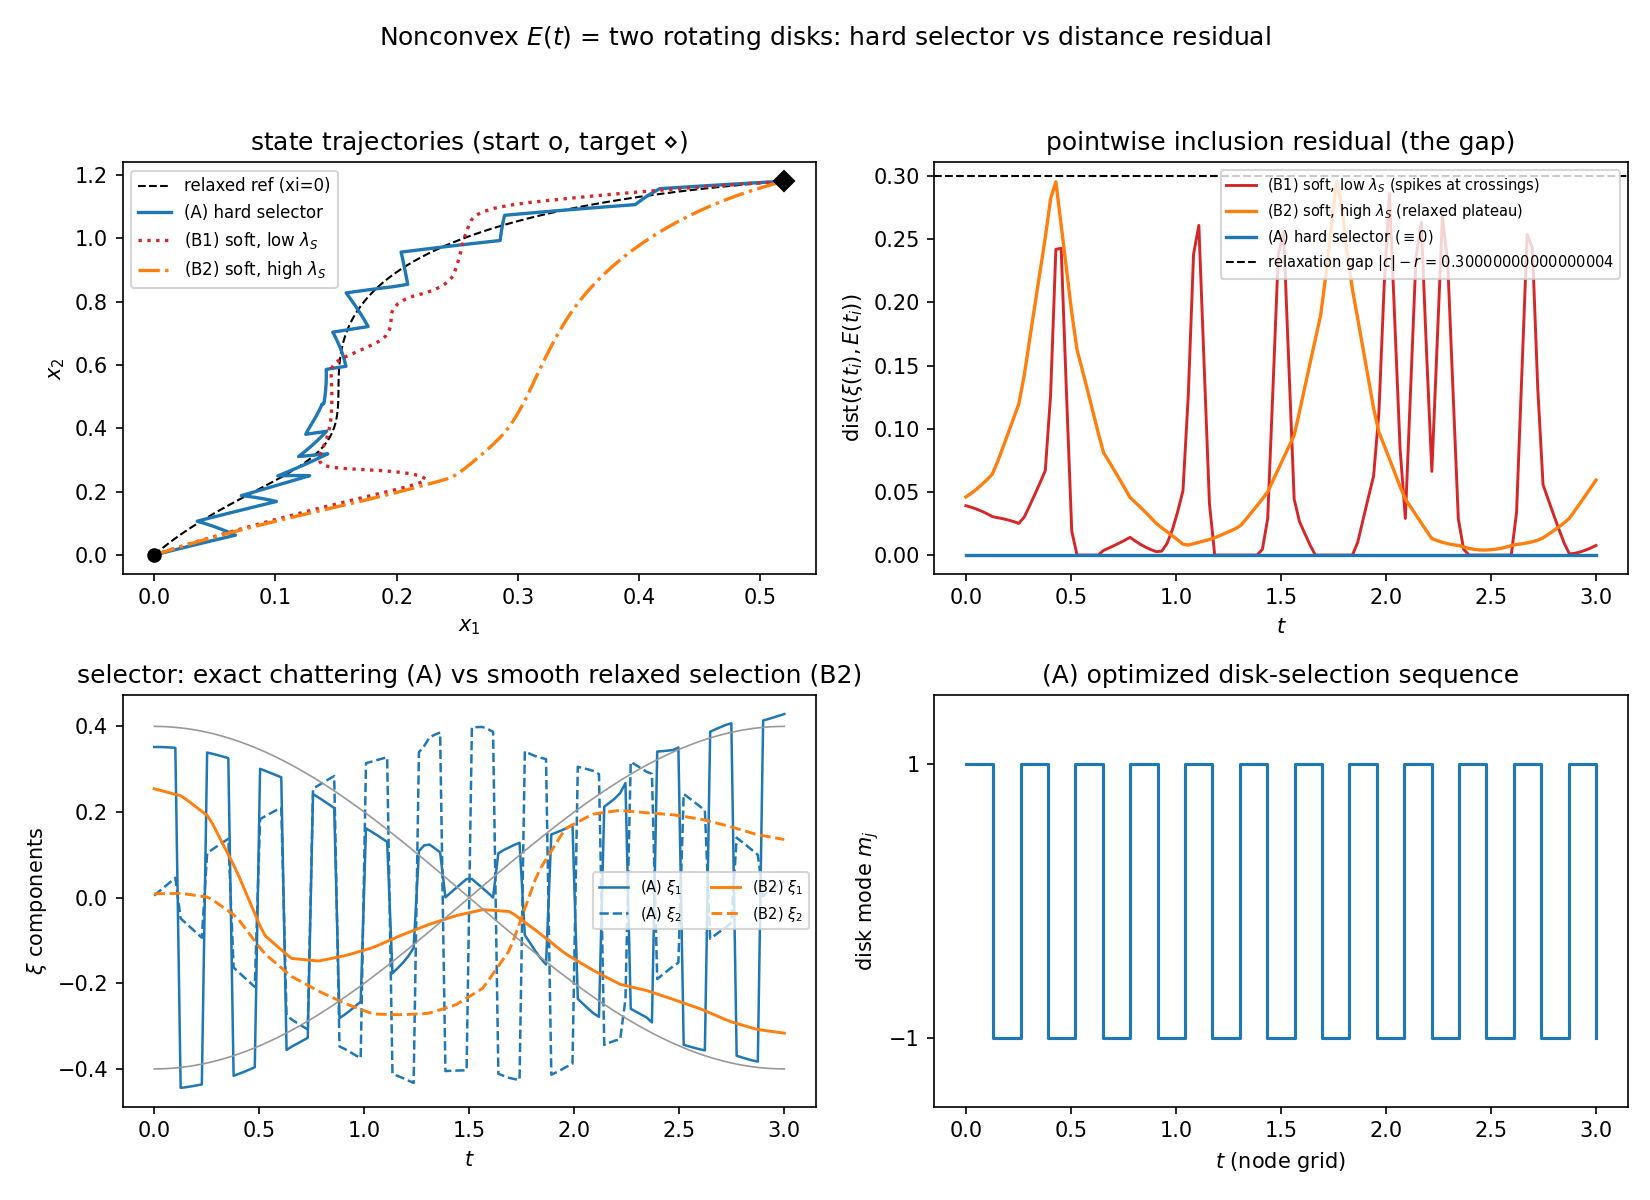
\includegraphics[width=\textwidth]{twodisk_relaxation_gap.png}
\caption{Nonconvex relaxation-gap experiment. Top left: all trajectories reach essentially the same target. Top right: the hard selector has zero residual, whereas the soft selectors exhibit crossing spikes or a relaxed plateau close to the gap scale $\delta=0.3$. Bottom left: the hard selector chatters between the two rotating components, while the strongly smoothed selector follows a relaxed path. Bottom right: the optimized hard mode sequence alternates between the two disks.}
\label{fig:results}
\end{figure}

For the weakly smoothed soft method, the selector attempts to switch between the two disks. Because it is represented by a continuous, finite-bandwidth interpolant, each switch crosses the forbidden gap and produces a residual spike approaching $\delta$. For the strongly smoothed method, rapid switching is too expensive, and the optimizer spends a positive fraction of the horizon between the disks. This produces a broad residual plateau. Which particular relaxed selector is obtained is optimizer-dependent; the endpoint is highly nonunique.

\section{Interpretation and limitations}

The benchmark separates four statements that are easily conflated.

\begin{enumerate}[label=(\roman*)]
\item \textbf{Pointwise exactness survives nonconvexity.} If the residual is exactly zero, the inclusion is satisfied because $E(t)$ is closed.

\item \textbf{The convex compactness proof does not survive.} The map $v\mapsto\dist^2(v,E(t))$ is nonconvex, and the integral residual is not weakly lower semicontinuous.

\item \textbf{A sequence of exact nonconvex solutions may converge to a non-solution.} Chattering solutions converge uniformly to the relaxed trajectory generated by $\xi=0$.

\item \textbf{Finite bandwidth creates a visible residual floor.} A smooth surrogate cannot realize arbitrarily fast switching. It must either cross the gap, creating spikes, or remain in the convexified region, creating a plateau.
\end{enumerate}

The numerical soft baseline is a collocation analogue of a DR-PINN, not yet a neural-network experiment. The smoothing term in \eqref{eq:soft_discrete} acts as a controlled proxy for the spectral bias of a smooth network. Replacing it by a tanh network would test the same geometry with an actual DR-PINN architecture.

\begin{remark}[Time-discretization detail]
The mathematically exact hard selector is \eqref{eq:hard_selector}, with the current rotating center $c(t)$ evaluated at every time, including all RK4 stages. In the supplied script, the complete sampled value $\xi_i$ is frozen during each RK4 step. Therefore, exact admissibility is guaranteed at the grid points, while between grid points there is an $O(\Delta t)$ mismatch because the disks continue to rotate. To obtain literal continuous-time admissibility in the implementation, one should freeze only the discrete mode and local disk coordinates, and reevaluate $m_jc(t)+r s(t)d(t)$ at each RK4 substage.
\end{remark}

\section{Conclusion}

The union of two rotating disks is a minimal nonconvex benchmark with an analytically known relaxation gap. It keeps the nonlinear, time-dependent drift and geometric control interpretation of the rotating-ellipse example, but introduces a disconnected admissible set. The hard hybrid parametrization handles this geometry exactly by combining a discrete mode with continuous within-disk coordinates. The distance-residual formulation remains computationally cheap because the distance is explicit, but its convex consistency proof no longer applies. The example therefore provides a direct numerical test of the transition from exact nonconvex dynamics to convexified relaxed dynamics and a clean way to measure that transition through the pointwise and mean inclusion residuals.

\begin{thebibliography}{9}
\bibitem{AubinCellina}
J.-P. Aubin and A. Cellina,
\emph{Differential Inclusions: Set-Valued Maps and Viability Theory},
Springer, 1984.

\bibitem{Deimling}
K. Deimling,
\emph{Multivalued Differential Equations},
De Gruyter, 1992.

\bibitem{Warga}
J. Warga,
\emph{Optimal Control of Differential and Functional Equations},
Academic Press, 1972.
\end{thebibliography}

\end{document}
